\documentclass[conference]{IEEEtran}
\IEEEoverridecommandlockouts
\usepackage{cite}
\usepackage{amsmath,amssymb}
\usepackage{graphicx}
\usepackage{booktabs}
\usepackage{algorithm}
\usepackage{algpseudocode}
\usepackage{tikz}
\usetikzlibrary{arrows.meta,positioning,fit}
\usepackage[hidelinks]{hyperref}
\usepackage{xcolor}
% generated by report/make_tables.py from results/ — do not edit
\newcommand{\TotalPatients}{53}
\newcommand{\TotalRows}{1015}
\newcommand{\TestRows}{206}
\newcommand{\TestExcluded}{0}
\newcommand{\TrainRows}{603}
\newcommand{\TestAccBase}{0.039}
\newcommand{\TestAccFT}{0.709}
\newcommand{\TestFoneBase}{0.077}
\newcommand{\TestFoneFT}{0.566}
\newcommand{\TestEvBase}{0.157}
\newcommand{\TestEvFT}{0.579}
\newcommand{\TestEvNonemptyFT}{0.747}
\newcommand{\TestWrong}{60}
\newcommand{\TopCell}{23}
\newcommand{\BestRun}{C: r16 + weights}
\newcommand{\BestEpoch}{4}
\newcommand{\BestValFone}{0.572}
\newcommand{\TrainableParams}{18.5}
\newcommand{\ValAccFT}{0.738}
\newcommand{\ValFoneFT}{0.527}
\newcommand{\KvMaxSpeedup}{20.3}
\newcommand{\KvMaxInput}{2048}
\newcommand{\KvCachedMs}{43}
\newcommand{\KvNoCacheMs}{875}
\newcommand{\KvFirstSpeedup}{1.2}
\newcommand{\AttnErrThirtyTwo}{1.8e-06}
\newcommand{\AttnErrSixteen}{4.9e-04}
\newcommand{\SdpaErrSixteen}{2.0e-03}
\newcommand{\AttnConfigs}{144}
\newcommand{\AttnLongSeq}{8192}
\newcommand{\AttnRefMB}{9280}
\newcommand{\AttnTiledMB}{29}
\newcommand{\AttnMemRatio}{317}
\newcommand{\InModelDiff}{0.13}
\newcommand{\SpecBaseStep}{47}
\newcommand{\SpecDraftMs}{40}
\newcommand{\SpecBestSpeedup}{0.93}
\newcommand{\SpecWorstSpeedup}{0.59}
\newcommand{\SpecAccMin}{0.59}
\newcommand{\SpecAccMax}{0.87}
\newcommand{\SpecHFcheck}{5/5}


\newcommand{\code}[1]{\texttt{\small #1}}
% TODO before submitting: replace with \url{<your video link>}
\newcommand{\VideoURL}{\textcolor{red}{[add video link]}}
\tikzset{box/.style={draw=black!70, rounded corners=1pt, align=center, font=\scriptsize, inner sep=3pt, minimum height=0.85cm, text width=1.55cm},
         arr/.style={-{Stealth[length=4pt]}, thick, black!70}}

\begin{document}

\title{TrialMatch: Criterion-Level Clinical Trial Screening with a Fine-Tuned 1.5B Language Model, an Own KV Cache, Tiled Attention and Speculative Decoding}

\author{\IEEEauthorblockN{Muhammad Rafique}
\IEEEauthorblockA{Roll no.\ 23i-0747 \textperiodcentered{} Section CS-B\\
Generative AI, Assignment 2}}

\maketitle

\begin{abstract}
We fine-tune an open-weight decoder, Qwen2.5-1.5B-Instruct, to judge one patient note against one clinical-trial criterion at a time, returning a label from the dataset's four-label set and the ids of the note sentences that support it. Training uses QLoRA on a 6\,GB laptop GPU and the expert annotations of the TrialGPT Criterion Annotations dataset, split by patient (37/8/8, seed 42). On the sealed test split the fine-tuned model reaches accuracy \TestAccFT{} and macro-F1 \TestFoneFT{}, against \TestAccBase{} and \TestFoneBase{} for the untrained model; evidence micro-F1 rises from \TestEvBase{} to \TestEvFT{}. Around the model we implement three inference components from scratch: a cache-aware greedy decoder (identical tokens to full recomputation, up to \KvMaxSpeedup$\times$ faster decoding at \KvMaxInput{} input tokens), tiled online-softmax attention (maximum fp32 error \AttnErrThirtyTwo{}, \AttnMemRatio$\times$ less working memory at \AttnLongSeq{} tokens) and greedy speculative decoding with a 0.5B draft (exactly the target's output, but \SpecWorstSpeedup--\SpecBestSpeedup$\times$ speed on this hardware, which we explain from measured draft and verify costs). A browser application exposes screening with evidence highlighting, a rule-based preliminary outcome and live benchmarks.
\end{abstract}

\begin{IEEEkeywords}
clinical trial matching, parameter-efficient fine-tuning, QLoRA, KV cache, online softmax, speculative decoding
\end{IEEEkeywords}

\section{Introduction}
Recruiting patients for clinical trials requires checking a patient's record against every inclusion and exclusion criterion of a protocol. TrialGPT~\cite{jin2024trialgpt} showed that a large proprietary model can make these criterion-level judgements and cite the sentences it relied on. This project asks whether a \emph{small, open} model, adapted on a laptop GPU, can learn the same task from expert annotations, and builds the inference machinery around it by hand.

The task is defined per criterion. Given a patient note split into numbered sentences, a criterion type (inclusion or exclusion) and the criterion text, the model returns JSON \code{\{"label": ..., "evidence\_ids": [...]\}}. Inclusion criteria take \emph{included}, \emph{not included}, \emph{not enough information} or \emph{not applicable}; exclusion criteria take \emph{excluded}, \emph{not excluded}, \emph{not enough information} or \emph{not applicable}. The two ``uncertain'' labels are kept as first-class answers rather than collapsed into a binary decision. An explanation is built from the cited sentences, never generated, and a patient-level outcome is derived by an explicit rule (Section~\ref{sec:app}) that is presented as a preliminary rule, not a prediction.

Contributions: (i) a reproducible patient-grouped split and evaluation protocol with explicit rules for empty evidence; (ii) a QLoRA sweep on a 6\,GB GPU with selection on validation only; (iii) own implementations of a KV-cached decoder, tiled online-softmax attention and greedy speculative decoding, each verified for exactness and benchmarked; (iv) a FastAPI and Next.js application for unseen notes.

\section{Related Work}
\textbf{Clinical eligibility.} TrialGPT~\cite{jin2024trialgpt} matches patients to trials with GPT-4 in three stages and reports 87.3\% criterion-level accuracy on the 1,015 expert-checked pairs we use; it relies on a paid API and is zero-shot. Wornow et al.~\cite{wornow2024zeroshot} also prompt large hosted models zero-shot, for inclusion criteria only. We instead adapt a 1.5B open model and measure the zero-shot version of that same model as the baseline.

\textbf{Architecture.} The decoder follows the Transformer~\cite{vaswani2017attention} with rotary position embeddings~\cite{su2021roformer} and grouped-query attention~\cite{ainslie2023gqa}; Qwen2.5~\cite{qwen2025} shares one tokenizer from 0.5B to 72B, which makes its 0.5B model a valid speculative draft for the 1.5B target.

\textbf{Adaptation.} LoRA~\cite{hu2022lora} learns low-rank updates to frozen weights; QLoRA~\cite{dettmers2023qlora} keeps the frozen base in 4-bit NF4, which is what makes training possible in 6\,GB.

\textbf{Efficient inference.} Pope et al.~\cite{pope2023scaling} separate compute-bound prefill from bandwidth-bound decode, which our benchmarks follow; PagedAttention~\cite{kwon2023paged} pages the KV cache for many concurrent requests, a design we considered and rejected for single-request use. Online softmax~\cite{milakov2018online} and FlashAttention~\cite{dao2022flash,dao2024flash2} compute exact attention block by block; we implement the algorithm but not the fused kernel, which explains our speed results. Speculative decoding~\cite{leviathan2023spec,chen2023specsampling} reduces to ``accept while the argmaxes agree'' under greedy decoding.

\section{Materials and Methods}

\subsection{Dataset and split}
We use the TrialGPT Criterion Annotations dataset~\cite{trialgptdata} (\TotalRows{} patient--criterion rows, \TotalPatients{} patients), pinned to revision \code{1cfcafde}. Only expert-written columns are kept through an explicit allow-list; all GPT-4 output columns are dropped so they can never leak into training or evaluation. Notes arrive as numbered sentences, which we parse rather than re-split so evidence ids stay aligned with the annotations. Patients are shuffled with NumPy's generator seeded at 42 and split 37/8/8, so no patient appears in two splits (Table~\ref{tab:split}). The split manifest with patient ids and file hashes is committed (\code{results/split\_manifest.json}). The splits are strongly imbalanced: \emph{not excluded} dominates exclusion rows, and the test split happens to contain \TestExcluded{} \emph{excluded} rows, so that label cannot be scored on test.

\begin{table*}[t]
\centering
\caption{Patient-grouped split (seed 42) and label counts per split.}
\label{tab:split}
\footnotesize
\setlength{\tabcolsep}{4pt}
\begin{tabular}{lrr|rrrr|rrrr}
\toprule
 & & & \multicolumn{4}{c|}{Inclusion} & \multicolumn{4}{c}{Exclusion} \\ Split & Pat. & Rows & inc & not inc & NEI & NA & exc & not exc & NEI & NA \\
\midrule
train & 37 & 603 & 88 & 13 & 109 & 5 & 8 & 292 & 65 & 23 \\
val & 8 & 206 & 35 & 3 & 27 & 1 & 2 & 101 & 26 & 11 \\
test & 8 & 206 & 27 & 7 & 38 & 3 & 0 & 91 & 28 & 12 \\
\bottomrule
\end{tabular}
\\[2pt]\parbox{0.95\linewidth}{\scriptsize Source: results/split\_manifest.json (dataset revision 1cfcafde94a1). NEI = not enough information, NA = not applicable.}
\end{table*}


\subsection{Model and prompt}
The target is Qwen2.5-1.5B-Instruct (28 layers, 12 query heads sharing 2 key/value heads, head size 128; \code{results/model\_candidates.json}); the draft is Qwen2.5-0.5B-Instruct, whose tokenizer we verified identical (\code{results/tokenizer\_compat.json}). The prompt (Fig.~\ref{fig:arch}) is a system message plus the numbered sentences, the criterion type, the criterion and the meaning of its four labels; the answer is the compact JSON object. The longest training example is 636 tokens, so nothing is truncated at the 1,024-token limit (\code{results/truncation\_report.json}). An unreadable answer is counted as a parse error, never guessed.

\begin{figure*}[t]
\centering
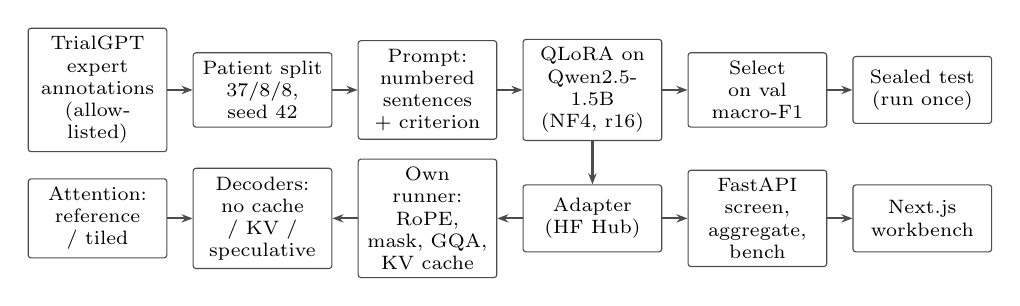
\begin{tikzpicture}[node distance=0.32cm]
\node[box] (data) {TrialGPT expert annotations\\(allow-listed)};
\node[box, right=of data] (split) {Patient split\\37/8/8, seed 42};
\node[box, right=of split] (prompt) {Prompt: numbered sentences + criterion};
\node[box, right=of prompt] (qlora) {QLoRA on Qwen2.5-1.5B\\(NF4, r16)};
\node[box, right=of qlora] (sel) {Select on val\\macro-F1};
\node[box, right=of sel] (test) {Sealed test\\(run once)};
\node[box, below=0.55cm of qlora] (adapter) {Adapter\\(HF Hub)};
\node[box, left=of adapter] (runner) {Own runner: RoPE, mask, GQA, KV cache};
\node[box, left=of runner] (dec) {Decoders: no cache / KV / speculative};
\node[box, left=of dec] (attn) {Attention: reference / tiled};
\node[box, right=of adapter] (api) {FastAPI\\screen, aggregate, bench};
\node[box, right=of api] (web) {Next.js workbench};
\draw[arr] (data) -- (split); \draw[arr] (split) -- (prompt); \draw[arr] (prompt) -- (qlora); \draw[arr] (qlora) -- (sel); \draw[arr] (sel) -- (test);
\draw[arr] (qlora) -- (adapter); \draw[arr] (adapter) -- (runner); \draw[arr] (runner) -- (dec); \draw[arr] (attn) -- (dec);
\draw[arr] (adapter) -- (api); \draw[arr] (api) -- (web);
\end{tikzpicture}
\caption{System architecture. Top: data and training pipeline. Bottom: inference; the merged adapter feeds our own runner, whose attention function and decoders are the Task~3--5 implementations, served by the API and the browser app.}
\label{fig:arch}
\end{figure*}

\subsection{Fine-tuning}
We train LoRA adapters on all attention and MLP projections (rank 16, $\alpha$=32, dropout 0.05; \TrainableParams{}\,M trainable parameters) over an NF4 base with double quantisation and bf16 compute~\cite{dettmers2023qlora}. The loss is cross-entropy on the answer tokens only (prompt tokens masked with $-100$). We use batch size 1 with 8-step gradient accumulation, AdamW (lr $2\times10^{-4}$, no weight decay), clipping at 1.0, and 5\% linear warm-up followed by cosine decay, for 5 epochs. To counter the label imbalance, one run weights each example's loss by the inverse square root of its (type, label) frequency, normalised to mean 1 and capped at 5. Four configurations (Table~\ref{tab:sweep}) were run overnight; after every epoch the adapter is saved, validation loss is computed and the validation split is decoded and scored. The best run and epoch by validation macro-F1 is chosen; the test split is never used for selection. The chosen adapter is published on the Hugging Face Hub (\code{Aduhere/trialmatch-qwen2.5-1.5b-qlora}).

\subsection{KV-cache decoding}
Our runner executes the Qwen2 stack layer by layer, reusing only the model's weights and its linear, normalisation and MLP modules; positions, masks, grouped-query attention and the cache are our code. The cache holds preallocated per-layer key/value buffers of shape $[2, L_{\max}, 128]$ and a length counter; \code{crop(n)} rolls it back (used by speculative decoding). New tokens are rotated at their absolute positions $\ell..\ell{+}T{-}1$, where $\ell$ is the cache length, before their keys are stored, so cached keys never need re-rotation~\cite{su2021roformer}. Query $i$ may attend to keys $0..\ell{+}i$. Algorithm~\ref{alg:kv} gives the cached greedy loop; the reference decoder instead re-runs the whole sequence from an empty cache at every step. The cache costs $2\cdot28\cdot2\cdot128\cdot2$ bytes = 28\,KB per token in fp16, growing linearly.

\begin{algorithm}[t]
\caption{Cache-aware greedy decoding}\label{alg:kv}
\small
\begin{algorithmic}[1]
\Require prompt ids $x_{1..P}$, max new tokens $n$, end token \textsc{eos}
\State $C \gets$ empty cache; $z \gets \textsc{Forward}(x_{1..P}, C)$ \Comment{prefill}
\State $y \gets [\arg\max z_P]$
\While{$|y| < n$ \textbf{and} $y_{\text{last}} \neq$ \textsc{eos}}
  \State $z \gets \textsc{Forward}(y_{\text{last}}, C)$ \Comment{1 token at position $|C|$}
  \State append $\arg\max z$ to $y$ \Comment{$C$ grew by one key/value per layer}
\EndWhile
\State \Return $y$
\end{algorithmic}
\end{algorithm}

\subsection{Tiled attention with an online softmax}
The reference attention materialises $S = QK^\top/\sqrt{d}$ in fp32, masks future keys with $-\infty$, subtracts each row's maximum before the exponential, and normalises; fully masked rows return zero instead of NaN. The tiled version (Algorithm~\ref{alg:tiled}) streams over key/value blocks and keeps, per query row, a running maximum $m$, normaliser $\ell$ and output accumulator $O$~\cite{milakov2018online,dao2022flash}. Under causal masking, key blocks entirely in the future of a query block are skipped. Only one $B_r\times B_c$ tile of scores exists at a time, in pure PyTorch with no fused kernel.

\begin{algorithm}[t]
\caption{Tiled causal attention, one query block}\label{alg:tiled}
\small
\begin{algorithmic}[1]
\Require $Q_b$ ($B_r$ rows), $K,V$, query offset $q_0$
\State $m \gets -\infty$, $\ell \gets 0$, $O \gets 0$
\For{each key block $(K_j, V_j)$ starting at $k_0$}
  \If{$k_0 > q_0 + B_r - 1$} \textbf{break} \Comment{all future}\EndIf
  \State $S \gets Q_b K_j^\top/\sqrt{d}$; mask future keys with $-\infty$
  \State $m' \gets \max(m, \mathrm{rowmax}(S))$; $P \gets e^{S - m'}$; $\alpha \gets e^{m - m'}$
  \State $\ell \gets \alpha\ell + \mathrm{rowsum}(P)$; \; $O \gets \alpha O + P V_j$; \; $m \gets m'$
\EndFor
\State \Return $O/\ell$ \Comment{rows with $\ell=0$ return 0}
\end{algorithmic}
\end{algorithm}

\subsection{Greedy speculative decoding}
Algorithm~\ref{alg:spec} runs two of our runners with their own caches. The draft proposes $\gamma$ tokens; the target scores the pending token plus all guesses in \emph{one} forward pass; guesses are accepted while they equal the target's argmax, then the target's own token is emitted (a correction, or a bonus token when all $\gamma$ matched). Both caches are cropped to the accepted length, so rejected guesses leave no trace and positions stay consistent. Every emitted token is the target's argmax given exactly its prefix, so the output equals plain greedy target decoding~\cite{leviathan2023spec}.

\begin{algorithm}[t]
\caption{Greedy speculative round}\label{alg:spec}
\small
\begin{algorithmic}[1]
\Require target cache $C_t$ (covers all but pending token $u$), draft cache $C_d$
\State $d_{1..\gamma} \gets$ greedy draft tokens from the draft model
\State $p_{0..\gamma} \gets \arg\max \textsc{Forward}_t([u, d_1..d_\gamma], C_t)$ \Comment{one pass}
\State $k \gets$ largest $k$ with $d_i = p_{i-1}$ for all $i \le k$
\State emit $d_{1..k}$ and $p_k$; \; \textsc{Crop}$(C_t)$, \textsc{Crop}$(C_d)$ to the accepted length
\end{algorithmic}
\end{algorithm}

\subsection{Application}\label{sec:app}
A FastAPI backend loads the fine-tuned model once (adapter merged into the fp16 base) and serves \code{/screen}, \code{/aggregate}, \code{/benchmark}, \code{/attention-bench}, \code{/report} and validation \code{/examples}; schema validation returns clear 422 errors, and GPU out-of-memory is caught. Unseen notes are split into sentences (a note already numbered ``0.\,1.\,\ldots'' is parsed as in training). The overall outcome follows a stated rule: any inclusion \emph{not included} or exclusion \emph{excluded} gives \emph{likely ineligible}; otherwise any \emph{not enough information} (or unreadable answer) gives \emph{needs review}; otherwise \emph{likely eligible}. The Next.js front end (Fig.~\ref{fig:app}) shows the note beside a case-report-form view in which every criterion displays all four possible answers with the model's ticked, the expert's answer circled on validation examples, and the cited sentences highlighted; a benchmark view runs the three decoders and the attention kernels live on the user's input. Fig.~\ref{fig:flow} shows one request end to end.

\begin{figure}[t]
\centering
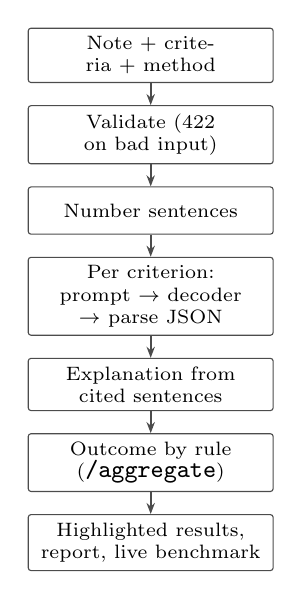
\begin{tikzpicture}[node distance=0.28cm, box/.append style={text width=2.9cm, minimum height=0.6cm}]
\node[box] (a) {Note + criteria + method};
\node[box, below=of a] (b) {Validate (422 on bad input)};
\node[box, below=of b] (c) {Number sentences};
\node[box, below=of c] (d) {Per criterion: prompt $\to$ decoder $\to$ parse JSON};
\node[box, below=of d] (e) {Explanation from cited sentences};
\node[box, below=of e] (f) {Outcome by rule (\code{/aggregate})};
\node[box, below=of f] (g) {Highlighted results, report, live benchmark};
\foreach \x/\y in {a/b,b/c,c/d,d/e,e/f,f/g} \draw[arr] (\x) -- (\y);
\end{tikzpicture}
\caption{Application workflow for one screening request.}
\label{fig:flow}
\end{figure}

\section{Experimental Setup and Metrics}
All runs use one NVIDIA RTX 3050 6\,GB laptop GPU, PyTorch 2.11 (CUDA 12.8), Transformers 5.22, PEFT 0.21 and bitsandbytes 0.50 on Windows 11. Evaluation decodes greedily with at most 64 new tokens. The evaluation runs of Tables~\ref{tab:test} and~\ref{tab:sweep} used the library's \code{generate}, which also applies the model's default repetition penalty of 1.1; Table~\ref{tab:penalty} shows this changes no label on validation and only the evidence lists. Our own decoders, used by the app and the benchmarks, are pure argmax.

Label metrics are accuracy, macro-F1 over labels present in the gold set, per-class precision/recall/F1 and confusion matrices, reported overall and per criterion type. Evidence is scored as sets of sentence ids: micro precision/recall/F1 over all rows, and macro F1 over rows; a row with empty gold and empty prediction is a correct abstention and is excluded from the macro average. Timings are wall-clock with \code{torch.cuda.synchronize()} around every phase, after one warm-up run, as means over 3--5 repeats; memory is \code{torch.cuda.max\_memory\_allocated} reset per run.

\section{Results and Discussion}

\subsection{Fine-tuning and model selection}
Table~\ref{tab:sweep} and Fig.~\ref{fig:curves} summarise the sweep. Label weighting gave the largest gain: run C improved macro-F1 over the unweighted run A almost entirely through the rare exclusion labels, which it begins to predict. Rank 8 matched rank 16, so adapter capacity was not the bottleneck. Validation loss reached its minimum at epoch 2 for the 2e-4 runs and then rose while macro-F1 kept improving (Fig.~\ref{fig:curves}): the model becomes more confident on frequent labels while still learning rare ones, so loss is not a good selection signal here. We selected run \BestRun{} at epoch \BestEpoch{} (validation macro-F1 \BestValFone{} with the 4-bit in-training model; \ValFoneFT{} re-scored with the fp16 base the app uses, the difference arising almost entirely from the two validation \emph{excluded} rows).

\begin{table*}[t]
\centering
\caption{QLoRA sweep, best epoch of each run by validation macro-F1 (4-bit, in-training scoring).}
\label{tab:sweep}
\footnotesize
\setlength{\tabcolsep}{4pt}
\begin{tabular}{lrrcr|rrrrr}
\toprule
Run & $r$ & LR & Wts & Ep. & Val loss & Acc & Macro-F1 & Excl F1 & Evid.\ F1 \\
\midrule
A: r16 & 16 & 0.0002 & no & 5 & 0.157 & 0.738 & 0.442 & 0.445 & 0.548 \\
B: r8 & 8 & 0.0002 & no & 5 & 0.157 & 0.743 & 0.443 & 0.427 & 0.555 \\
C: r16 + weights & 16 & 0.0002 & yes & 4 & 0.159 & 0.757 & 0.572 & 0.622 & 0.517 \\
D: r16, lr 5e-5 & 16 & 5e-05 & no & 5 & 0.138 & 0.757 & 0.528 & 0.560 & 0.575 \\
\bottomrule
\end{tabular}
\\[2pt]\parbox{0.95\linewidth}{\scriptsize Source: results/train\_*/summary.json. Wts = inverse-square-root label weighting.}
\end{table*}


\begin{figure}[t]
\centering
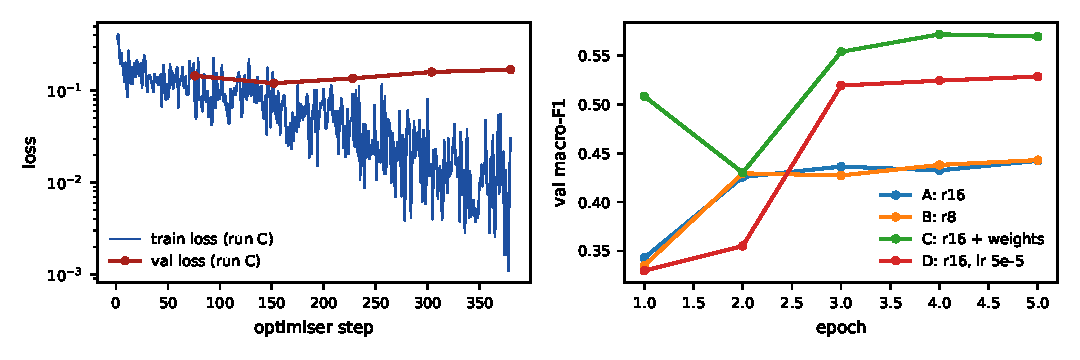
\includegraphics[width=\linewidth]{figures/train_curves.pdf}
\caption{Training curves. Left: per-step training loss and per-epoch validation loss for the selected run C. Right: validation macro-F1 per epoch for the four runs (source: \code{results/train\_*/}).}
\label{fig:curves}
\end{figure}

\subsection{Test results: before and after fine-tuning}
Table~\ref{tab:test} compares the untrained and fine-tuned models on the same \TestRows{} test criteria. The untrained model produces valid JSON but collapses to one label per criterion type and reads exclusion criteria with inverted polarity (its exclusion accuracy is zero). Fine-tuning raises accuracy from \TestAccBase{} to \TestAccFT{} and macro-F1 from \TestFoneBase{} to \TestFoneFT{}, with no parse errors. Evidence micro-F1 rises from \TestEvBase{} to \TestEvFT{}, and to \TestEvNonemptyFT{} on rows where the expert cited at least one sentence. With 206 items the 95\% interval on accuracy is roughly $\pm$6 points, so differences of a few points against other runs are within noise. Per class (Table~\ref{tab:perclass}), frequent labels (\emph{included}, \emph{not excluded}) and inclusion \emph{not enough information} score well; the rare \emph{not included} and exclusion \emph{not enough information} remain weak, which the confusion matrices in Fig.~\ref{fig:conf} make visible.

\begin{table*}[t]
\centering
\caption{Sealed test split, untrained (left of each pair) vs fine-tuned (right). Same 206 criteria, same prompt and decoding.}
\label{tab:test}
\footnotesize
\setlength{\tabcolsep}{4pt}
\begin{tabular}{lr|rr|rr|rr|rr|r}
\toprule
Subset & $n$ & \multicolumn{2}{c|}{Accuracy} & \multicolumn{2}{c|}{Macro-F1} & \multicolumn{2}{c|}{Evid.\ micro-F1} & \multicolumn{2}{c|}{Evid.\ macro-F1} & Parse err. \\
\midrule
overall & 206 & 0.039 & 0.709 & 0.077 & 0.566 & 0.157 & 0.579 & 0.061 & 0.460 & 0 / 0 \\
inclusion & 75 & 0.107 & 0.733 & 0.099 & 0.541 & 0.217 & 0.626 & 0.065 & 0.559 & 0 / 0 \\
exclusion & 131 & 0.000 & 0.695 & 0.000 & 0.487 & 0.137 & 0.478 & 0.059 & 0.264 & 0 / 0 \\
\bottomrule
\end{tabular}
\\[2pt]\parbox{0.95\linewidth}{\scriptsize Source: results/baseline\_test/metrics.json, results/finetuned\_test/metrics.json. Macro-F1 averages labels present in the gold set; evidence F1 compares cited sentence ids.}
\end{table*}

\begin{table}[t]
\centering
\caption{Per-class results on the test split (FT = fine-tuned).}
\label{tab:perclass}
\footnotesize
\setlength{\tabcolsep}{4pt}
\resizebox{\ifdim\width>\linewidth\linewidth\else\width\fi}{!}{%
\begin{tabular}{llr|rr|rr}
\toprule
Type & Label & Supp. & F1 base & F1 FT & P FT & R FT \\
\midrule
inc. & included & 27 & 0.312 & 0.792 & 0.905 & 0.704 \\
inc. & not included & 7 & 0.000 & 0.182 & 0.250 & 0.143 \\
inc. & not enough information & 38 & 0.000 & 0.791 & 0.708 & 0.895 \\
inc. & not applicable & 3 & 0.082 & 0.400 & 0.500 & 0.333 \\
exc. & excluded & 0 & -- & -- & -- & -- \\
exc. & not excluded & 91 & 0.000 & 0.818 & 0.741 & 0.912 \\
exc. & not enough information & 28 & 0.000 & 0.200 & 0.333 & 0.143 \\
exc. & not applicable & 12 & 0.000 & 0.444 & 0.667 & 0.333 \\
\bottomrule
\end{tabular}}
\\[2pt]\parbox{0.98\linewidth}{\scriptsize Source: per\_class in results/*\_test/metrics.json. ``--'': label absent from the test gold set.}
\end{table}


\begin{figure}[t]
\centering
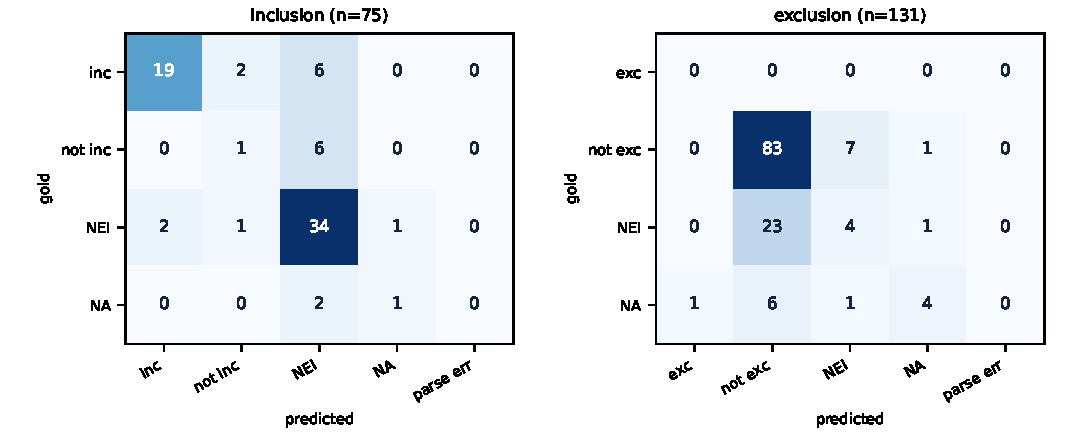
\includegraphics[width=\linewidth]{figures/confusion.pdf}
\caption{Fine-tuned model confusion matrices on test, inclusion (left) and exclusion (right) criteria (source: \code{results/finetuned\_test/}).}
\label{fig:conf}
\end{figure}

\subsection{Error analysis}
The fine-tuned model makes \TestWrong{} label errors on test. The largest cells (Table~\ref{tab:conf}) reveal the main failure: \TopCell{} exclusion criteria labelled \emph{not excluded} where the expert chose \emph{not enough information}, i.e.\ the model treats a condition the note never mentions as absent. We traced ten cases to their sentence ids (\code{results/error\_analysis.md}), including: absent evidence read as proof (``patients were moribund'', a hypotensive patient labelled not excluded); clinical implications missed (``tachycardic'' not recognised as heart rate $\geq$\,90); a negated criterion confused with a related procedure (arterial catheterisation read as central venous); a label contradicting the model's own correctly cited evidence (an SLE patient with malar rash and swollen joints labelled \emph{not included}); temporal and frequency conditions ignored (snoring without the required three-month history accepted); confusion between \emph{not applicable} and \emph{not enough information} for sex- and age-dependent criteria; and over-citing background sentences when abstaining, the most common evidence-only error. Two cases show contradictory gold annotations: the experts themselves label ``not mentioned'' as \emph{not excluded} for some criteria and \emph{not enough information} for others, and label a pregnancy criterion for a 48-year-old man \emph{not excluded} where a boy's equivalent is \emph{not applicable}. Part of the residual error is therefore annotation inconsistency rather than model error; we report the gold labels unchanged.

\begin{table}[t]
\centering
\caption{Largest error cells of the fine-tuned model on test.}
\label{tab:conf}
\footnotesize
\setlength{\tabcolsep}{4pt}
\resizebox{\ifdim\width>\linewidth\linewidth\else\width\fi}{!}{%
\begin{tabular}{lll}
\toprule
Count & Gold & Predicted \\
\midrule
23 & not enough information & not excluded \\
7 & not excluded & not enough information \\
6 & not included & not enough information \\
6 & not applicable & not excluded \\
6 & included & not enough information \\
\bottomrule
\end{tabular}}
\\[2pt]\parbox{0.98\linewidth}{\scriptsize Source: confusion matrix in results/finetuned\_test/metrics.json.}
\end{table}

\begin{table}[t]
\centering
\caption{Validation: generate's default repetition penalty (1.1) vs pure greedy (1.0).}
\label{tab:penalty}
\footnotesize
\setlength{\tabcolsep}{4pt}
\resizebox{\ifdim\width>\linewidth\linewidth\else\width\fi}{!}{%
\begin{tabular}{llrrr}
\toprule
Model & Rep.\ pen. & Acc & Macro-F1 & Evid.\ F1 \\
\midrule
untrained & 1.1 & 0.068 & 0.081 & 0.134 \\
untrained & 1.0 & 0.068 & 0.081 & 0.091 \\
fine-tuned & 1.1 & 0.738 & 0.527 & 0.507 \\
fine-tuned & 1.0 & 0.738 & 0.527 & 0.547 \\
\bottomrule
\end{tabular}}
\\[2pt]\parbox{0.98\linewidth}{\scriptsize Source: results/\{baseline,finetuned\}\_val\{,\_greedy\}/metrics.json. No label changed in any of the 206 rows.}
\end{table}


\subsection{KV cache}
Cached decoding produced exactly the same tokens as both our full-recompute decoder and the library's uncached forward at 64/32, 256/64 and 1024/128 input/output tokens. Table~\ref{tab:kv} and Fig.~\ref{fig:kv} show the benefit growing with prompt length: without the cache each new token costs about one prefill (\KvNoCacheMs{}\,ms at \KvMaxInput{} tokens), with the cache it stays near \KvCachedMs{}\,ms, from \KvFirstSpeedup$\times$ at 128 tokens to \KvMaxSpeedup$\times$ at \KvMaxInput{}. Cached decode is bound by reading the 3\,GB of weights and launching small kernels, so its cost per token is almost independent of length. Peak memory barely differs because the weights dominate and the cache adds only 28\,KB per token.

\begin{table}[t]
\centering
\caption{KV-cache benchmark, 64 new tokens, mean of 5 runs after warm-up.}
\label{tab:kv}
\footnotesize
\setlength{\tabcolsep}{4pt}
\resizebox{\ifdim\width>\linewidth\linewidth\else\width\fi}{!}{%
\begin{tabular}{rrrrrrr}
\toprule
Input & Prefill ms & ms/tok no cache & ms/tok cache & Speed-up & Peak GB & Cache MB \\
\midrule
128 & 50 & 58.5 & 50.6 & 1.2$\times$ & 2.90 / 2.90 & 5.2 \\
512 & 150 & 163.6 & 40.6 & 4.0$\times$ & 2.95 / 2.94 & 15.7 \\
1024 & 327 & 346.4 & 38.7 & 9.0$\times$ & 3.05 / 3.04 & 29.7 \\
2048 & 808 & 874.7 & 43.1 & 20.3$\times$ & 3.41 / 3.38 & 57.7 \\
\bottomrule
\end{tabular}}
\\[2pt]\parbox{0.98\linewidth}{\scriptsize Source: results/bench/kvcache.json. Token equality with full recomputation at 64/32, 256/64, 1024/128 (input/output): all identical.}
\end{table}


\begin{figure*}[t]
\centering
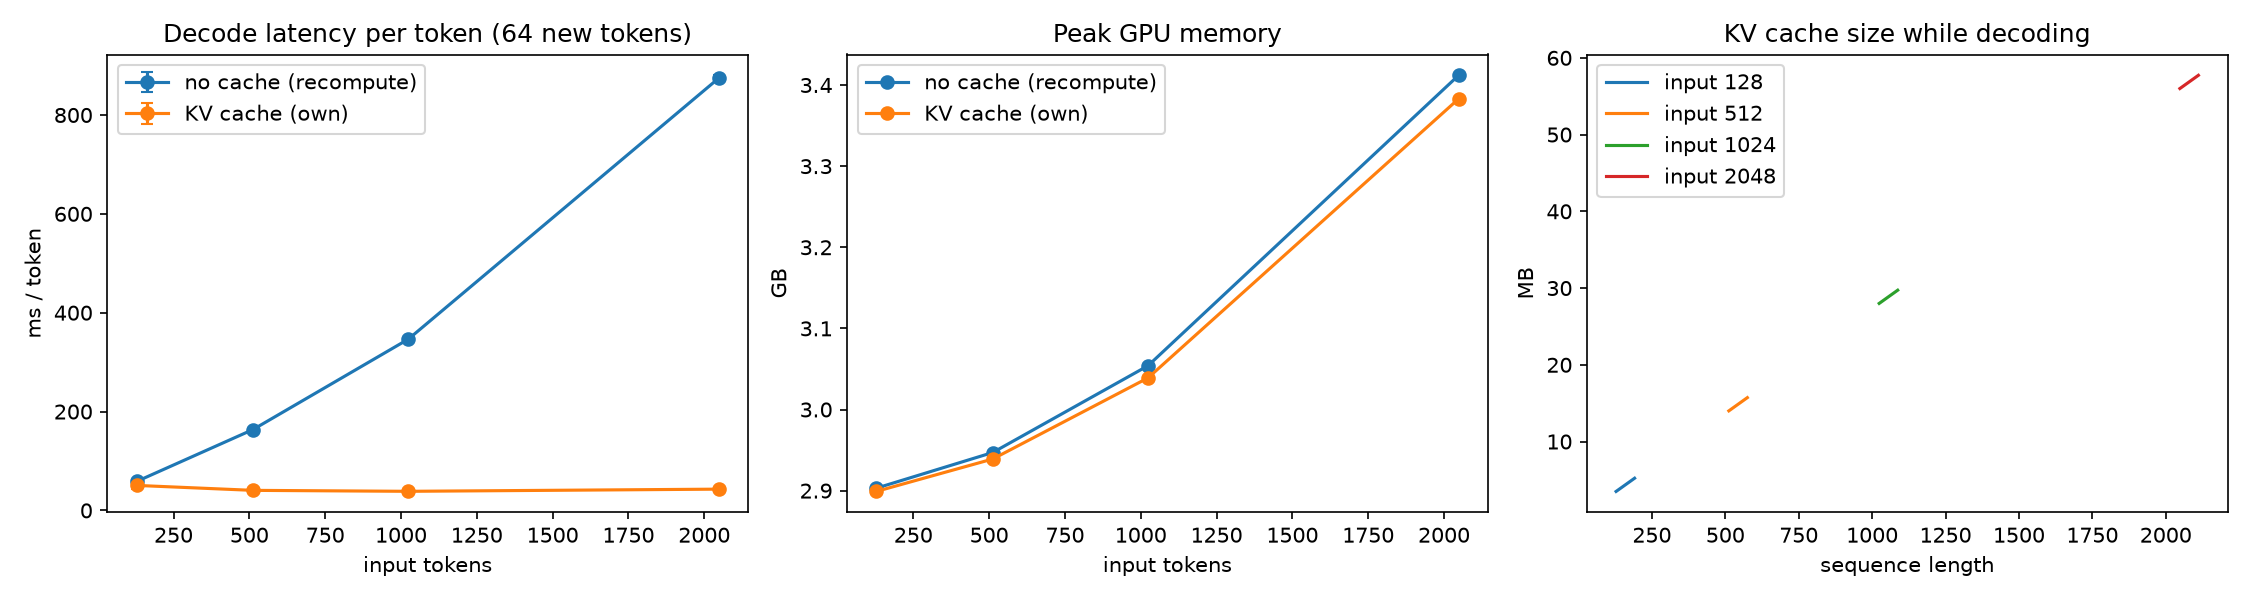
\includegraphics[width=0.95\linewidth]{figures/kvcache.png}
\caption{KV-cache benchmark: decode latency per token, peak memory, and cache size while decoding (source: \code{results/bench/kvcache.json}).}
\label{fig:kv}
\end{figure*}

\subsection{Tiled attention}
Over \AttnConfigs{} configurations (sequence lengths up to 2,048, head sizes 32--128, causal and non-causal, two block shapes) the tiled kernel matched the reference to at most \AttnErrThirtyTwo{} in fp32 and \AttnErrSixteen{} in fp16, closer than PyTorch's fp16 SDPA (\SdpaErrSixteen{}), because it accumulates in fp32 and rounds once. Replacing attention in all 28 layers of the model changed prefill logits by at most \InModelDiff{} and left 64 greedy tokens identical. Table~\ref{tab:attn} and Fig.~\ref{fig:attn} show the trade-off: at \AttnLongSeq{} tokens the reference needs \AttnRefMB{}\,MB of working memory (beyond the 6\,GB card, so Windows spilled it to system memory) while the tiled version needs \AttnTiledMB{}\,MB, about \AttnMemRatio$\times$ less, growing linearly rather than quadratically. Our tiling is slower than the fused kernels because each tile is a series of separate kernel launches from a Python loop with every intermediate round-tripping through GPU main memory; PyTorch's memory-efficient kernel performs the same tiling on-chip and obtains both the memory saving and the speed.

\begin{table}[t]
\centering
\caption{Attention time (ms) / extra memory (MB), causal, 12 heads, $d{=}128$, fp16.}
\label{tab:attn}
\footnotesize
\setlength{\tabcolsep}{4pt}
\resizebox{\ifdim\width>\linewidth\linewidth\else\width\fi}{!}{%
\begin{tabular}{rrrrr}
\toprule
Seq & Reference & Tiled ($B{=}128$) & SDPA math & SDPA mem-eff. \\
\midrule
256 & 4.6 / 9 & 5.4 / 6 & 5.9 / 13 & 0.4 / 1 \\
512 & 18.5 / 36 & 18.4 / 7 & 4.9 / 40 & 0.4 / 2 \\
1024 & 12.8 / 145 & 49.6 / 8 & 11.9 / 136 & 2.4 / 3 \\
2048 & 40.6 / 580 & 157.0 / 11 & 42.7 / 496 & 1.8 / 6 \\
4096 & 153.0 / 2320 & 645.5 / 17 & 136.0 / 1888 & 7.3 / 12 \\
8192 & 5086.9 / 9280 & 2651.6 / 29 & 1464.1 / 7360 & 26.9 / 24 \\
\bottomrule
\end{tabular}}
\\[2pt]\parbox{0.98\linewidth}{\scriptsize Source: results/bench/attention.json (1 warm-up, 5 repeats). The flash SDPA backend is absent from the Windows PyTorch build.}
\end{table}


\begin{figure*}[t]
\centering
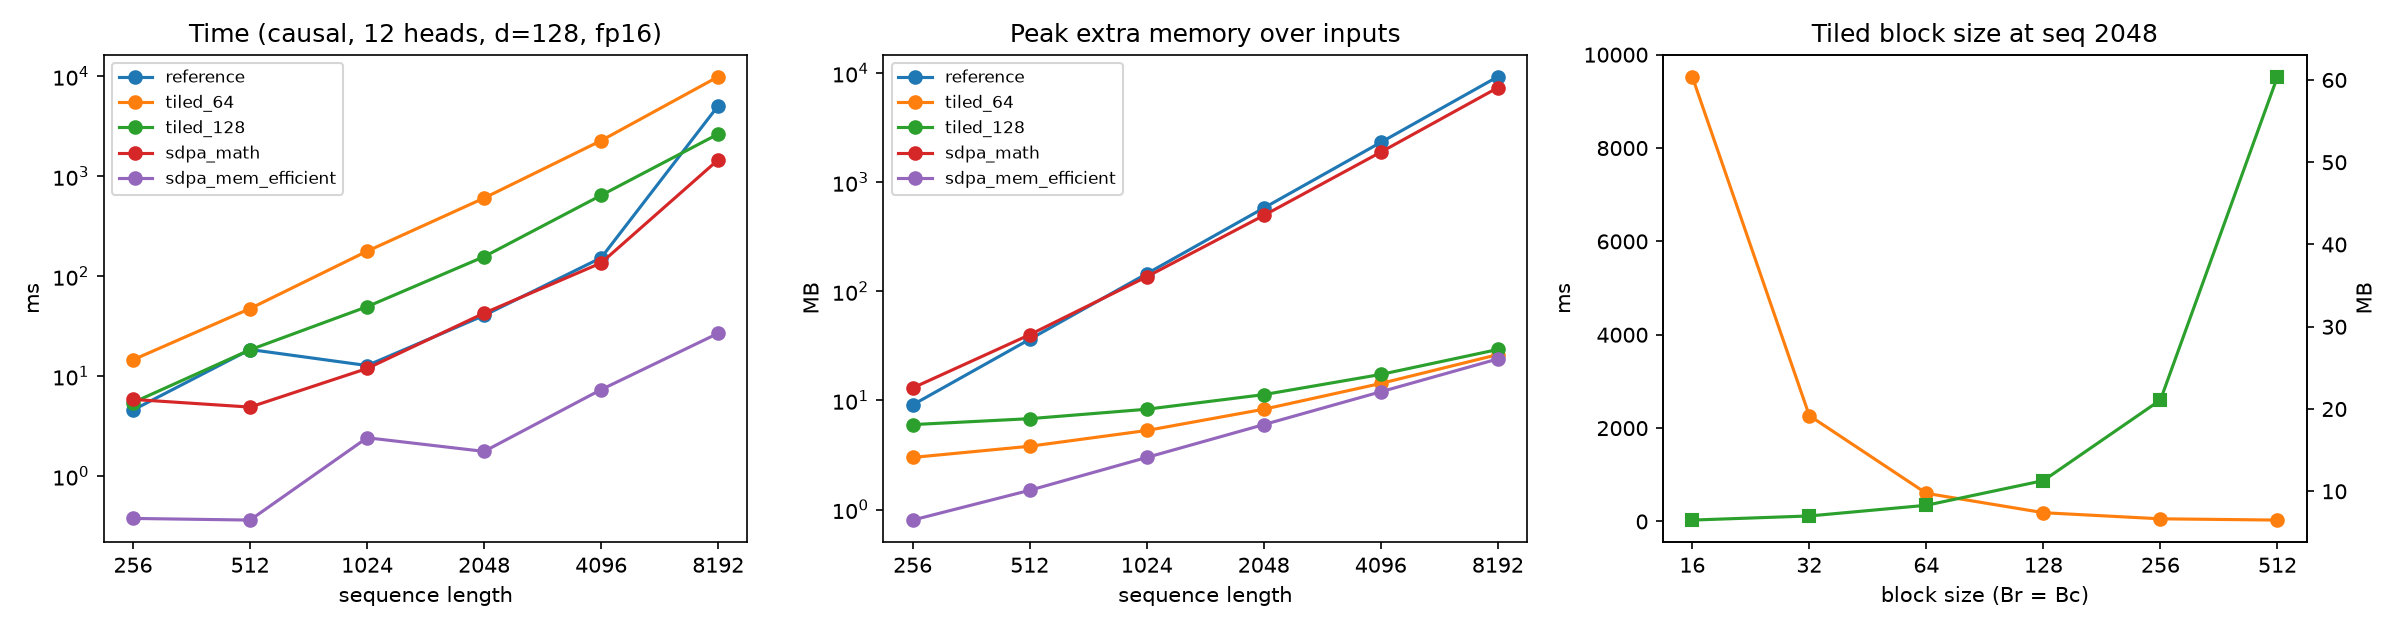
\includegraphics[width=0.95\linewidth]{figures/attention.png}
\caption{Attention benchmark: time and extra memory versus sequence length, and the tiled block-size trade-off at 2,048 tokens (source: \code{results/bench/attention.json}).}
\label{fig:attn}
\end{figure*}

\subsection{Speculative decoding}
Speculative output was identical to plain greedy decoding on every screening prompt at every $\gamma$, and to the library's assisted generation on \SpecHFcheck{} prompts; the single mismatch in a free-text workload was an exact fp16 tie (top-two logit gap 0.0000) broken differently by the one-token and multi-token kernels. Table~\ref{tab:spec} and Fig.~\ref{fig:spec} show that the draft is accepted \SpecAccMin--\SpecAccMax{} of the time and that verification works as intended: checking $\gamma{+}1$ tokens costs about one target step (\SpecBaseStep{}\,ms). The speed-up nevertheless stays below one (\SpecWorstSpeedup--\SpecBestSpeedup$\times$) because a draft step costs \SpecDraftMs{}\,ms, about 85\% of a target step: in our launch-bound runner cost scales with the number of layers (24 vs 28), not with model width. A cost model with draft/target ratio $c$, speed-up $\approx$ tokens-per-pass$/(\gamma c + 1)$, reproduces the measured trend; the same acceptance rates with $c = 0.1$ would give about 2$\times$. The fine-tuned target also lowers acceptance relative to the base target, since the untuned draft does not anticipate the compact JSON style.

\begin{table}[t]
\centering
\caption{Speculative decoding, fine-tuned target, 20 screening prompts (plain greedy: 19.8 tok/s).}
\label{tab:spec}
\footnotesize
\setlength{\tabcolsep}{4pt}
\resizebox{\ifdim\width>\linewidth\linewidth\else\width\fi}{!}{%
\begin{tabular}{rrrrrrrr}
\toprule
$\gamma$ & Accept & Tok/pass & Draft ms & Verify ms & tok/s & Speed-up & Identical \\
\midrule
1 & 0.869 & 1.74 & 40 & 47 & 18.4 & 0.93$\times$ & 20/20 \\
2 & 0.772 & 2.15 & 78 & 47 & 16.4 & 0.83$\times$ & 20/20 \\
3 & 0.810 & 2.67 & 117 & 47 & 16.2 & 0.82$\times$ & 20/20 \\
4 & 0.744 & 3.11 & 159 & 47 & 15.8 & 0.80$\times$ & 20/20 \\
6 & 0.650 & 3.46 & 229 & 50 & 13.6 & 0.69$\times$ & 20/20 \\
8 & 0.593 & 3.73 & 309 & 49 & 11.7 & 0.59$\times$ & 20/20 \\
\bottomrule
\end{tabular}}
\\[2pt]\parbox{0.98\linewidth}{\scriptsize Source: results/bench/speculative.json (1 warm-up, 3 repeats). Speed-up = plain cached greedy time / speculative time.}
\end{table}


\begin{figure*}[t]
\centering
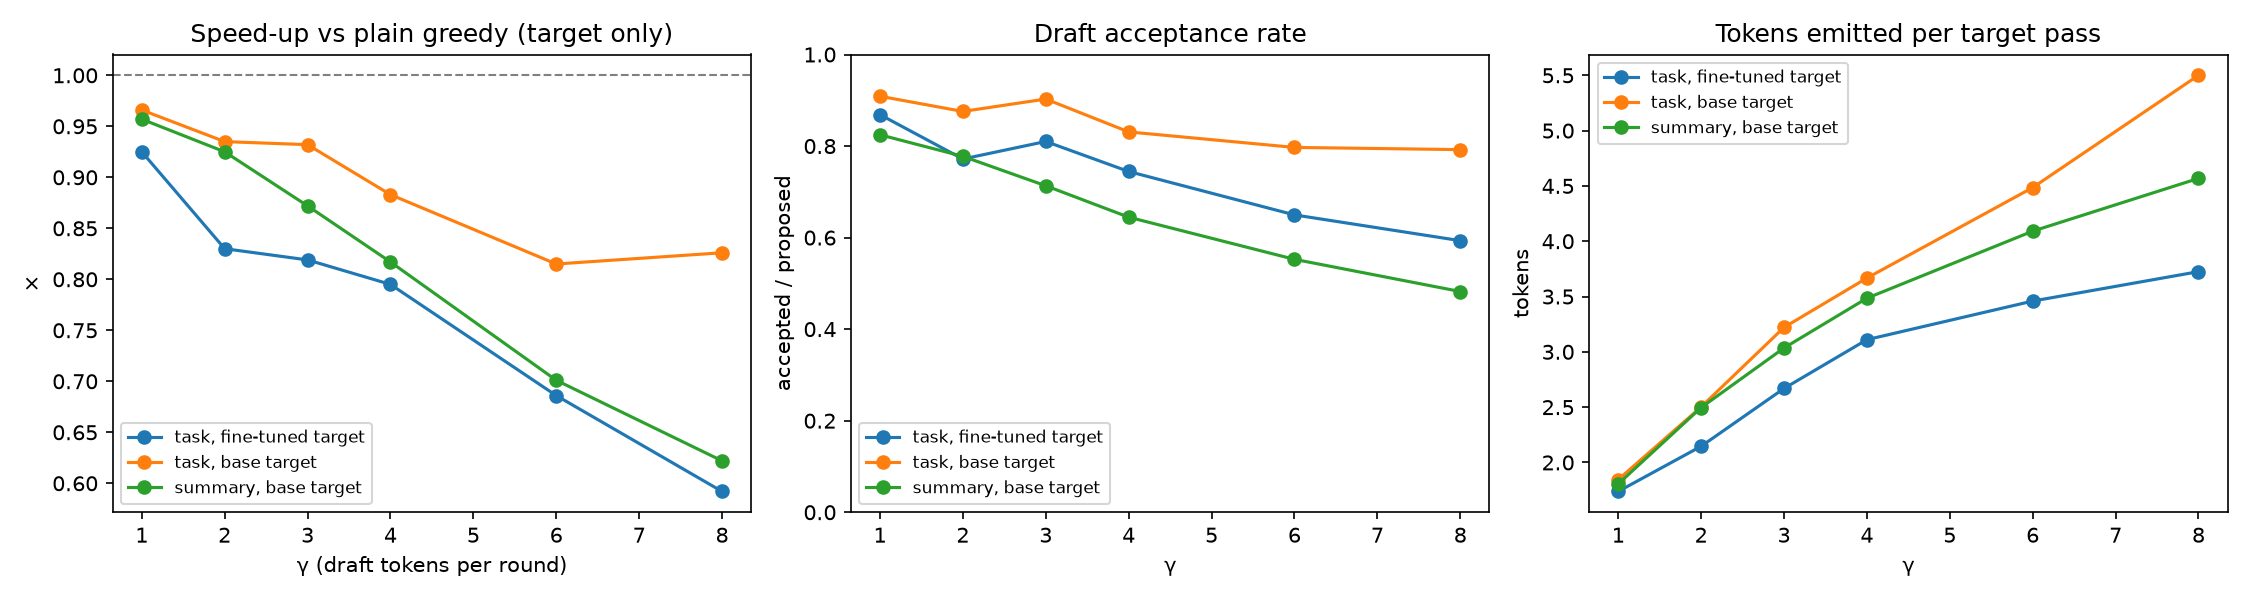
\includegraphics[width=0.95\linewidth]{figures/speculative.png}
\caption{Speculative decoding versus $\gamma$: speed-up over plain greedy, draft acceptance, and tokens emitted per target pass (source: \code{results/bench/speculative.json}).}
\label{fig:spec}
\end{figure*}

\subsection{Application}
Fig.~\ref{fig:app} shows the screening view on a validation example: the selected criterion's cited sentence is highlighted in the note, each sentence lists the criteria that cite it, the model's answer is ticked among all four, the expert's answer is circled (with an inline note where they disagree), and the outcome is shown with the rule that produced it. The benchmark view runs all three decoders on the same input and reports identical answers with their measured timings.

\begin{figure*}[t]
\centering
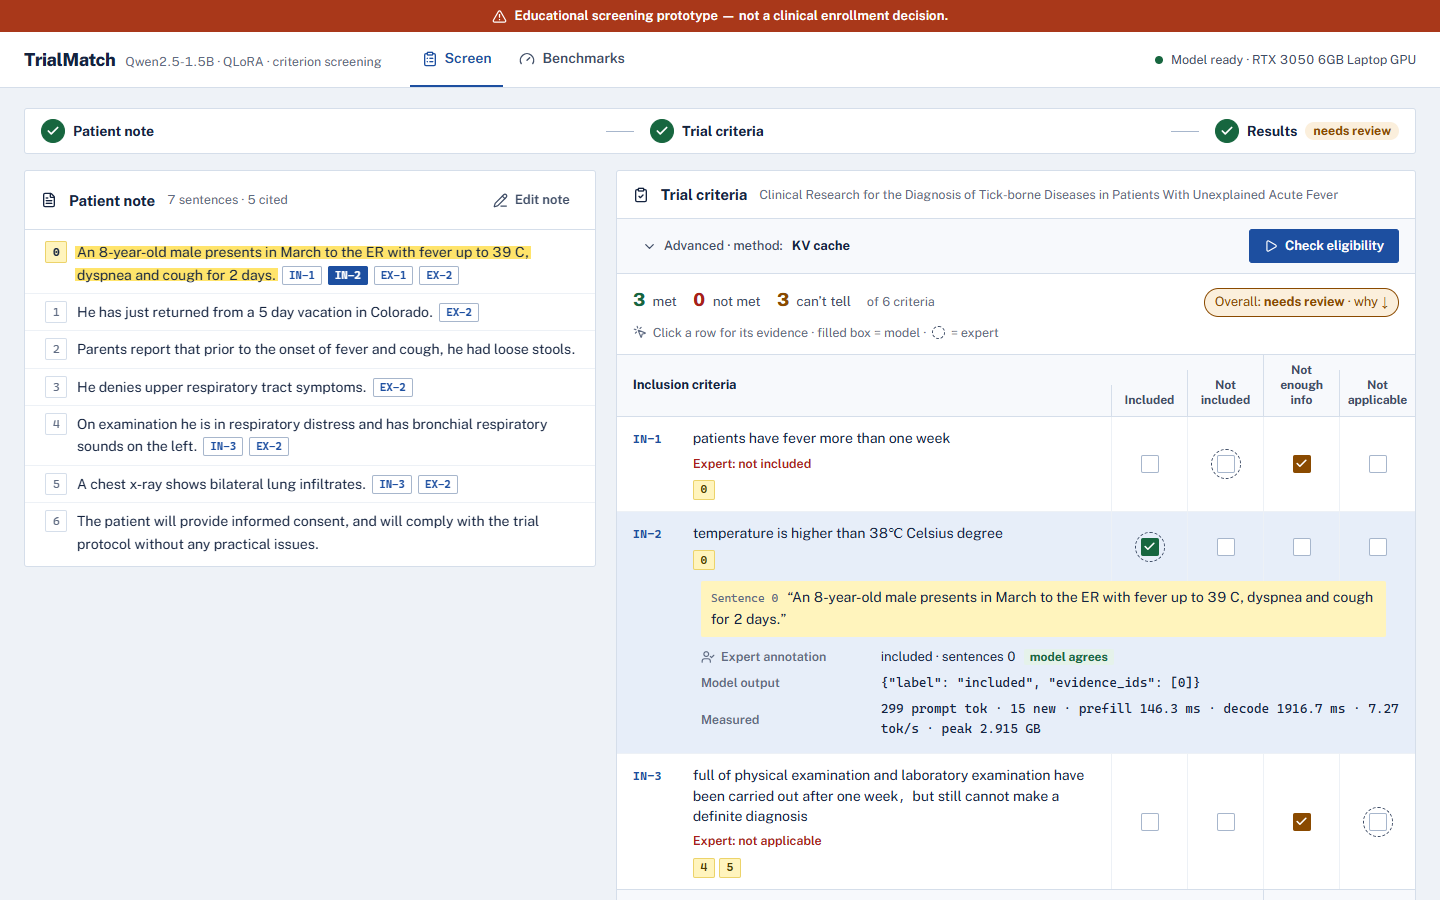
\includegraphics[width=0.49\linewidth]{figures/app_screen.png}\hfill
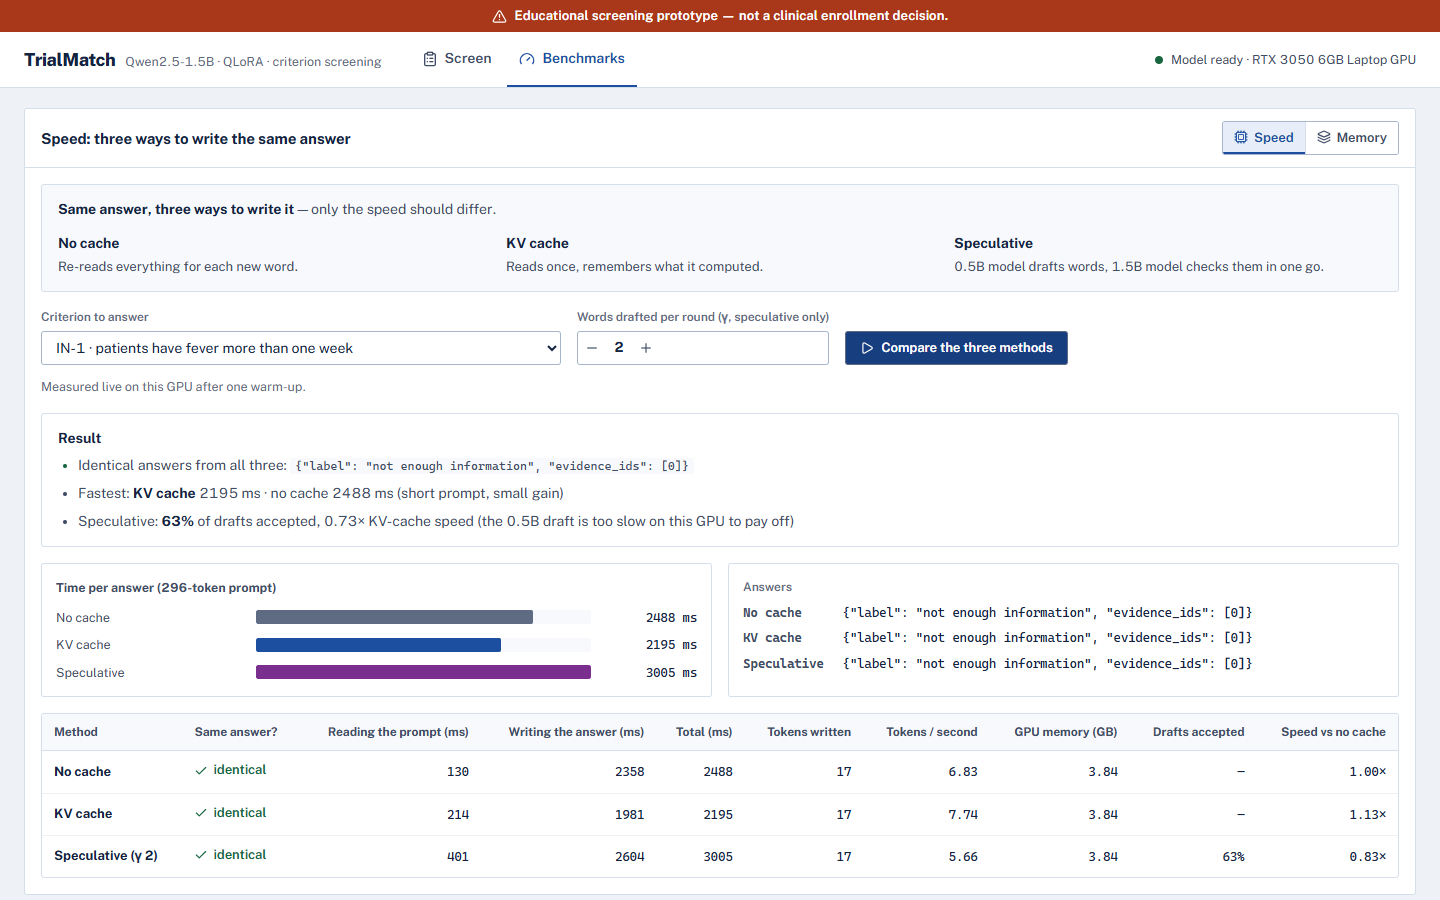
\includegraphics[width=0.49\linewidth]{figures/app_bench.png}
\caption{Application: screening view with evidence highlighting and expert comparison (left); live decoder comparison on the same input (right). Captured on battery power, so the displayed timings are throttled.}
\label{fig:app}
\end{figure*}

\section{Limitations}
The training set is small (\TrainRows{} rows from 37 patients) and stylistically narrow (emergency-department case vignettes), so notes written differently are out of distribution. The test split contains no \emph{excluded} row, so that label is untested, and with 206 items the accuracy interval is about $\pm$6 points. Annotation conventions for unmentioned conditions are inconsistent, which bounds achievable agreement. The evaluation decoding included the library's default repetition penalty (labels unaffected on validation, evidence lists slightly so). Our attention and speculative implementations demonstrate correctness and memory behaviour but not speed, because they are not fused kernels; speculative decoding did not pay off on this GPU. The patient-level outcome is a rule over predicted labels, not a validated prediction, and one wrong criterion can flip it. The system is an educational prototype and must not be used for clinical enrollment decisions.

\section{Code, Data and Demonstration}
Source code, the split manifest, training and benchmark logs: \url{https://github.com/Rafique610/trialmatch}. Fine-tuned adapter: \url{https://huggingface.co/Aduhere/trialmatch-qwen2.5-1.5b-qlora}. Demonstration video: \VideoURL. A fresh clone reproduces the split (identical manifest), the tests and the application with five commands listed in the repository README.

\section{Conclusion}
A 1.5B open model fine-tuned with QLoRA on a 6\,GB laptop GPU learns criterion-level eligibility judgements with cited evidence, improving test accuracy from \TestAccBase{} to \TestAccFT{} and macro-F1 from \TestFoneBase{} to \TestFoneFT{}. Our own KV cache, tiled attention and speculative decoder are exact by construction and verified token for token; the cache gives large decode speed-ups for long prompts, tiling gives large memory savings, and speculative decoding shows, with measurements, why a draft must be much cheaper than the target to help. Future work: more diverse training notes, a consistent convention for unmentioned conditions, and fused kernels for the attention and decoding paths.

\bibliographystyle{IEEEtran}
\bibliography{refs}

\appendices
\section{AI-use statement}
An AI coding assistant (Anthropic's Claude, used through Claude Code) helped write code, tests, documentation and this report's first draft under the author's direction. Every step was planned on a task board, reviewed and approved by the author before being committed. Design aids (the \emph{impeccable} and \emph{ui-ux-pro-max} skills and Google Stitch) were used to explore the interface; designs proposing invented figures were not adopted. All experiments were run by the author on the stated hardware, and every number in this paper is generated from the result files in the repository by \code{report/make\_tables.py}. No GPT-4 outputs from the dataset were used for training or evaluation.

\end{document}
